% !TEX root = ../popl-paper.tex

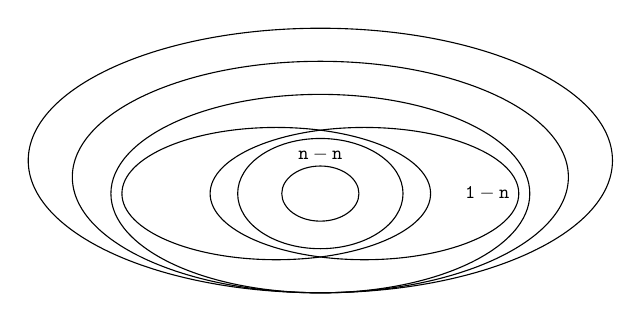
\begin{tikzpicture}[scale=0.7, every node/.style={transform shape}]
   % \draw (0,0) ellipse (5cm and 3cm);
    %\draw (0,0) ellipse (5cm and 3cm);
    %\draw (0,0) ellipse (5cm and 3cm);

\draw(0,0) ellipse (.7cm and .5cm); 
\node (r) at (0,0) {$\rsc$}; 
\draw(0,0) ellipse (1.5cm and 1cm); 
\node (nn) at (0,.7) {$\mathtt{n-n}$}; 

\draw(.8,0) ellipse (2.8cm and 1.2cm); 
\node[left] (n1) at (3.55,0) {$\mathtt{1-n}$}; 
\draw(-.8,0) ellipse (2.8cm and 1.2cm); 
\node[right] (1n) at (-3.5,0) {$\none$}; 

\draw(0,0) ellipse (3.8cm and 1.8cm); 
\node (nn) at (0,1.5) {$\co$}; 

\draw(0,.3) ellipse (4.5cm and 2.1cm); 
\node (nn) at (0,2) {$\oneone$}; 

\draw(0,.6) ellipse (5.3cm and 2.4cm); 
\node (nn) at (0,2.6) {$\asy$}; 

\end{tikzpicture} 

% \begin{tikzpicture}[inclusion/.style={right hook->, thick}]
%     \node (RSC)    at (-1.7,0) {\begin{tabular}{c}synchronous \\ (RSC)\end{tabular}};
%     \node (FIFOnn) at (1,0)  {\begin{tabular}{c}FIFO \\ n-n\end{tabular}}; 
%     \node (FIFO1n) at (3.2,1.5)  {\begin{tabular}{c}FIFO 1-n\end{tabular}};
%     \node (mb)     at (3.2,-1.5) {\begin{tabular}{c}FIFO n-1\\ (mailbox)\end{tabular}};
%     \node (co)     at (5.8,0)  {\begin{tabular}{c}causally\\ ordered\end{tabular}};
%     \node (p2p)    at (8,0) {\begin{tabular}{c}FIFO 1-1\\ (p2p)\end{tabular}};
%     \node (async)  at (10.4,0) {\begin{tabular}{c}asyn-\\ chronous\end{tabular}};
%     \draw[inclusion] (RSC) to (FIFOnn);
%     \draw[inclusion] (FIFOnn.north east) to (FIFO1n.west);
%     \draw[inclusion] (FIFOnn.south east) to (mb.west);
%     \draw[inclusion] (FIFO1n.east) to (co.north west);
%     \draw[inclusion] (mb.east) to (co.south west);
%     \draw[inclusion] (co) to (p2p);
%     \draw[inclusion] (p2p) to (async);
% \end{tikzpicture}